\chapter{Architettura del Software}

Il software è stato progettato in maniera modulare e scalabile per poter essere facilmente esteso e mantenuto.
Per raggiungere tale obiettivo è stata adottata un'architettura a microservizi in cui ogni servizio svolge un compito specifico e ben definito.

Per la connessione dei dispositivi embedded tra loro e con gli utenti è stato ideato un sistema federato attraverso il quale:
\begin{itemize}
    \item i dispositivi connessi allo stesso servizio comunicano tra loro in modo sicuro e diretto;
    \item i dispositivi connessi ad un servizio sono in grado di comunicare con dispositivi connessi ad altri servizi, a condizione che essi siano tra loro federati.
\end{itemize}

Inoltre, vista la necessità degli utenti di creare e gestire in maniera estremamente flessibile i propri device, il servizio client deve
seguire codice arbitrario fornito dall'utente in modo da aggiungere nuove funzionalità e personalizzare il comportamento del proprio dispositivo.

Seguono nel dettaglio i fondamenti teorici utilizzati per implementare il sistema.

\newpage

\section{Architettura Federata} 

\begin{figure}[h]
    \centering
    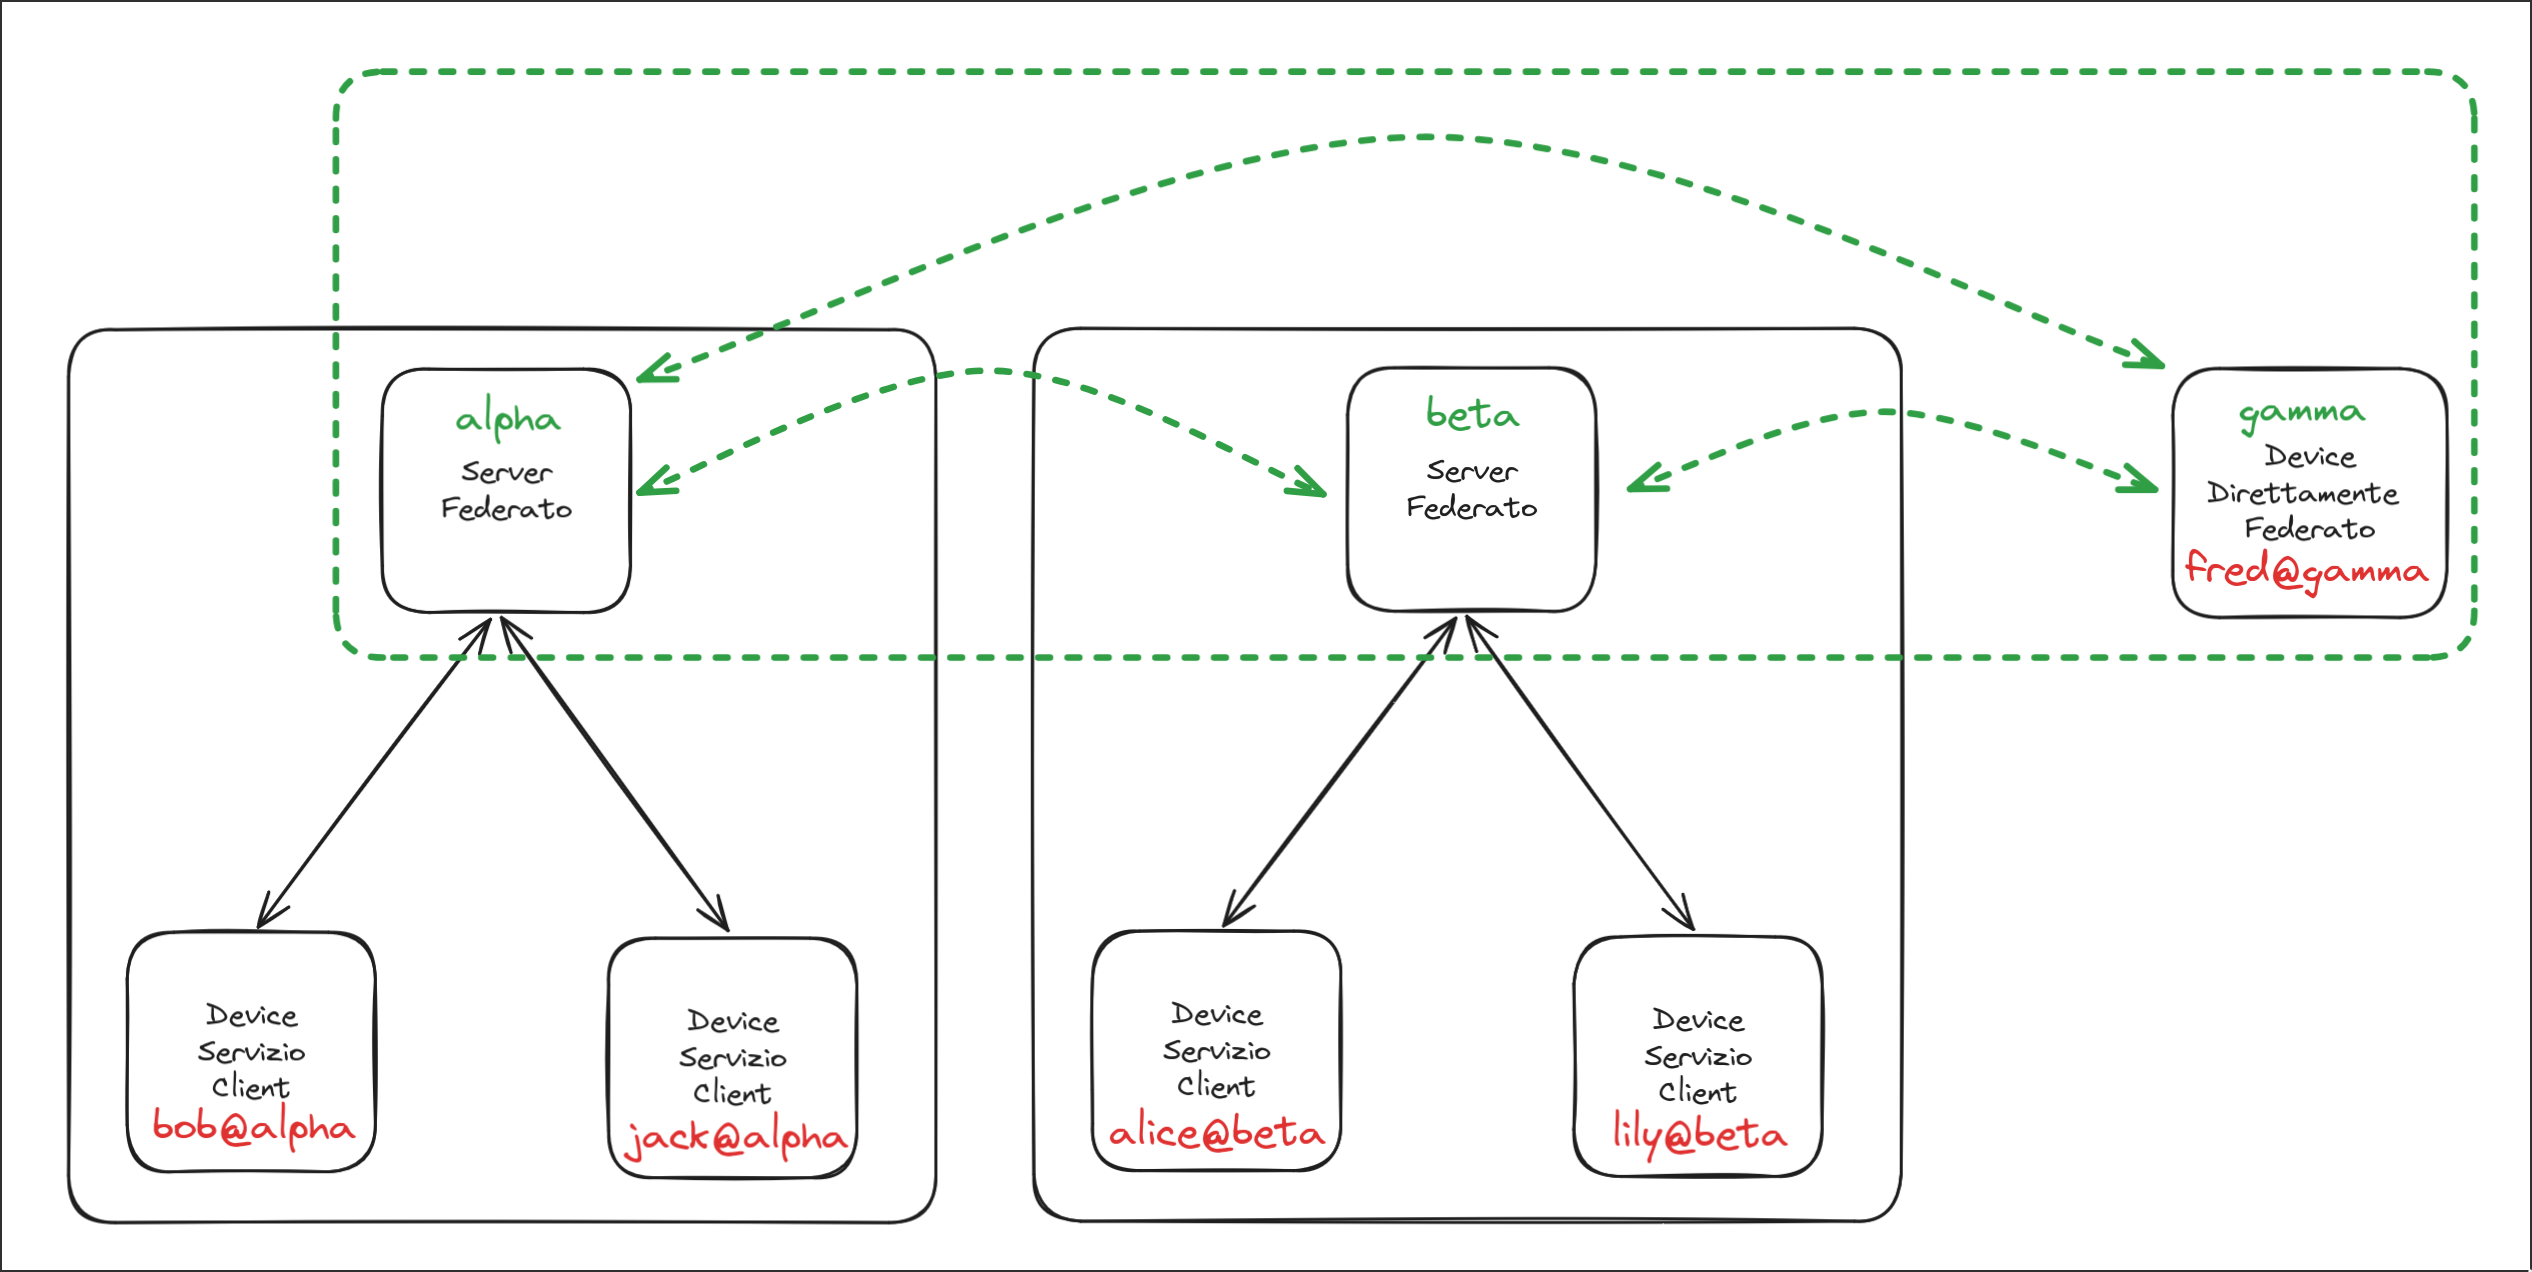
\includegraphics[width=1.0\textwidth]{images/chapter3/federation.png}
    \caption{Architettura federata}
    \label{fig:federated_architecture}
\end{figure}

Nella figura \ref{fig:federated_architecture} si nota che i device che eseguono il servizio client comunicano
con tutti gli altri device connessi alla rete federata tramite una connessione ad un server federato.
Questo tipo di server si occupa di instradare i messaggi tra i device garantendo che solo quelli autorizzati possano comunicare tra loro.
Se un dispositivo vuole comunicare con un altro che non è connesso allo stesso server federato, il messaggio viene instradato attraverso il server del device di destinazione.

Ogni device viene identificato da un codice univoco formato dal nome del dispositivo, una chiocciola (@) e il nome del server di appartenenza.
In aggiunta, il device può funzionare da server federato per consentire ad altri dispositivi di connettersi direttamente ad esso.

Il nome del server non è altro che un indirizzo IP o un nome di dominio che identifica il server federato all'interno della rete Internet,
mentre il nome del dispositivo è un identificativo scelto dall'utente ed è unico solamente all'interno del server federato.

È possibile quindi che esistano due device con lo stesso nome ma appartenenti a server federati diversi.

\section{Schema di sicurezza}

Le connessioni tra i device e i server federati sono crittografate mediante l'utilizzo del protocollo TLS in modo da garantire la riservatezza e l'integrità dei dati scambiati.
I device vengono autenticati dai server federati per consentire loro di comunicare in modo sicuro.

Tuttavia, l'esecuzione di codice arbitrario comporta un elevato rischio di sicurezza e per tale motivo si richiede 
un sistema di sandboxing per eseguire codice in un ambiente isolato e sicuro.

\subsection{Autenticazione}

\begin{figure}[H]
  \centering
  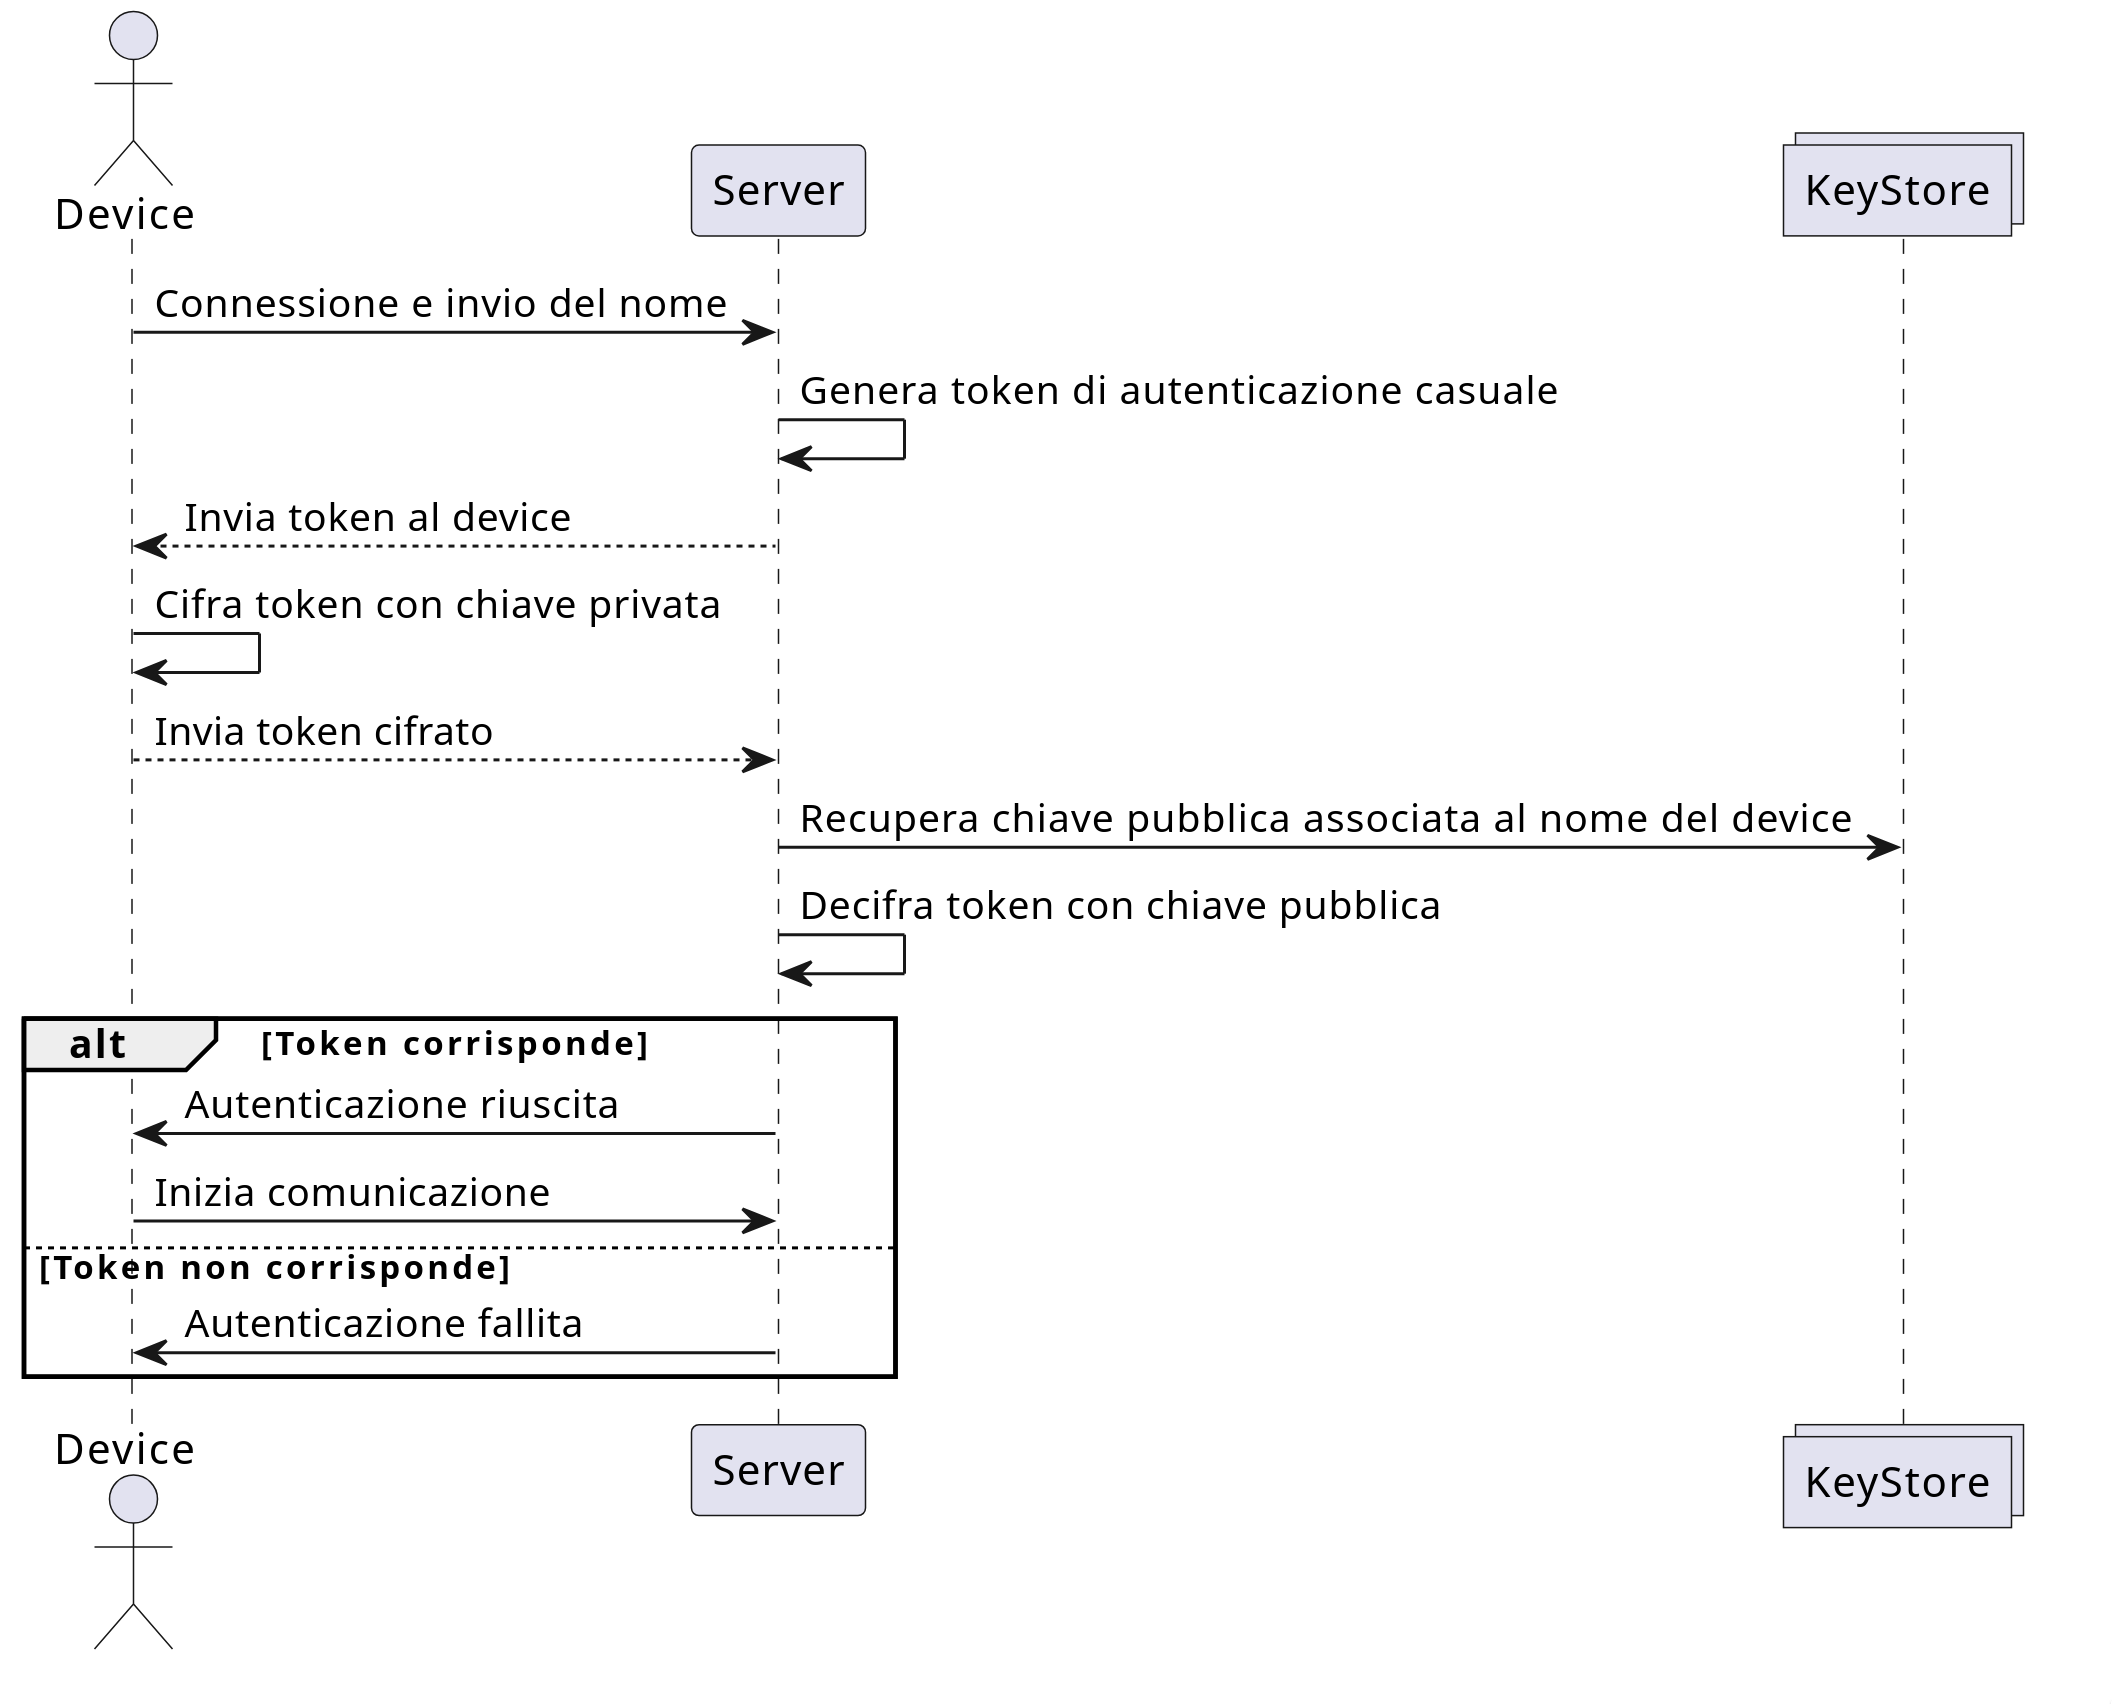
\includegraphics[width=1.0\textwidth]{images/chapter3/auth.png}
  \caption{Diagramma di sequenza dell'autenticazione}
  \label{fig:authentication_sequence}
\end{figure}

Il device si connette al server federato inviando il proprio nome e successivamente il server inizia il processo di autenticazione di tipo challenge-response.
Il server genera un token di autenticazione casuale e lo invia al device il quale lo cifra con una chiave privata e lo invia nuovamente al server che a sua volta
lo decifra con la chiave pubblica. Nel caso in cui il token decifrato corrisponda a quello generato in precedenza, il device viene autenticato correttamente e potrà comunicare con il server.
Un device può essere inoltre registrato su più server federati - i server al momento della federazione scambieranno le chiavi pubbliche per permettere la comunicazione tra i device.

\subsection{Sandboxing}

Eseguire codice arbitrario presenta un enorme rischio di sicurezza in quanto i device embedded sono spesso collegati alla reti di casa, aziendali, o addirittura a reti critiche come quelle di un ospedale.
La compromissione del dispositivo potrebbe portare a gravi conseguenze come il controllo di macchinari industriali o la violazione della sicurezza della rete.
È estremamente importante garantire che il codice eseguito all'interno del device non possa accedere a risorse sensibili o compromettere la sicurezza del sistema.
A tal fine sono stati esplorati due modi per implementare il sandboxing: l'utilizzo di macchine virtuali oppure l'interpretazione di un linguaggio di scripting.

In questa sezione si analizzano i punti di forza e le debolezze di entrambe le soluzioni. Successivamente 
vengono testate in maniera pratica al fine di scegliere la soluzione migliore.

\subsubsection{Virtual Machine}

Una macchina virtuale è un software che emula un computer reale e permette di eseguire un sistema operativo all'interno di un altro sistema operativo.
Normalmente, una macchina virtuale è isolata dal sistema operativo host e non può accedere alle sue risorse di sistema quali 
la memoria, il disco e la rete.

Nei computer general purpose, le macchine virtuali sono di facile implementazione grazie alle moderne CPU dotate 
di MMU~\cite{olivieri2022land} (Memory Management Unit), un hardware specifico che consente di creare un ambiente di memoria isolato per ogni applicativo.

\subparagraph{Vantaggi}

Implementare una semplice macchina virtuale richiede relativamente poco codice minimizzando la superficie di 
attacco, il che rende immediato testare il codice all'interno di un emulatore prima di eseguirlo sul dispositivo reale.
Nel caso venga implementato un instruction set preesistente come ad esempio quello RISC-V o ARM, sarà possibile
utilizzare toolchain predefinite per compilare codice proveniente da diversi linguaggi di programmazione di più alto livello
come C, C++ o Rust.

\subparagraph{Svantaggi}

La maggior parte dei microcontrollori embedded non possiede una MMU e ciò rende l'esecuzione di una macchina virtuale molto più lenta: 
ogni singola istruzione macchina deve essere emulata dal software, accrescendo notevolmente il tempo di esecuzione.
La macchina virtuale esegue solo codice macchina, è quindi necessario compilare il codice sorgente in codice macchina 
prima di poterlo eseguire, step che potrebbe risultare complicato per utenti poco esperti.

\subsubsection{Interpreter}

Un interprete è un software che legge un programma scritto in un linguaggio di programmazione di alto livello e lo esegue istruzione per istruzione.
Noti esempi di interpreti sono CPython per il linguaggio Python e il motore V8 per JavaScript.

\subparagraph{Vantaggi}

Programmare in un linguaggio di alto livello può risultare più semplice e veloce rispetto alla programmazione in linguaggio macchina o un in linguaggio di basso livello.
È possibile offrire quindi un'esperienza di programmazione più user-friendly in modo da permettere anche a persone non esperte di programmare il proprio device.

\subparagraph{Svantaggi}

Gli interpreti sono spesso molto più complessi di una macchina virtuale in quanto devono effettuare il parsing del codice sorgente,
generare un AST (Abstract Syntax Tree) ed infine interpretare le istruzioni.
Questo comporta un aumento della dimensione del firmware che potrebbe non essere accettabile per dispositivi con
risorse limitate, inoltre l'interpretazione del codice è più lenta rispetto all'esecuzione diretta del codice macchina.
Per via della complessità e della mole di codice richiesta dall'interprete, la superficie di attacco aumenta notevolmente.

\subsubsection{Scelta Tecnologica}

Si è deciso di testare 3 soluzioni per capire quale sia la più adatta per il progetto:
\begin{itemize}
    \item \texttt{rvsim}~\cite{rvsim} : una macchina virtuale RISC-V scritta in Rust;
    \item \texttt{Micropython}~\cite{micropython} : un interprete per il linguaggio Python per microcontrollori scritto in C;
    \item \texttt{rhai}~\cite{rhai_website}: un interprete e linguaggio di scripting scritto in Rust.
\end{itemize}

\begin{table}[H]
    \centering
    \begin{tabular}{|c|c|c|c|}
        \hline
        \textbf{Soluzione} & \textbf{Interoperabilità} & \textbf{Velocità} & \textbf{Semplicità d'uso} \\
        \hline
        \texttt{rvsim} & 
        \begin{tabular}[c]{@{}c@{}}- Buona \\ - è possibile creare \\ syscall custom \end{tabular} & 
        \begin{tabular}[c]{@{}c@{}}- Elevata \\ - codice compilato \end{tabular} & 
        \begin{tabular}[c]{@{}c@{}}- Difficile \\ - Richiede compilazione \\ del codice\end{tabular} \\
        \hline
        \texttt{Micropython} & 
        \begin{tabular}[c]{@{}c@{}}- Scarsa \\ - difficile da integrare \end{tabular} & 
        \begin{tabular}[c]{@{}c@{}}- Buona \\ - utilizza bytecode \end{tabular} & 
        \begin{tabular}[c]{@{}c@{}}- Semplice \\ - linguaggio semplice\\ molto diffuso \end{tabular} \\
        \hline
        \texttt{rhai} & 
        \begin{tabular}[c]{@{}c@{}}- Elevata \\ - supporto a funzioni \\ e tipi custom \end{tabular} & 
        \begin{tabular}[c]{@{}c@{}}- Scarsa \\ - poco ottimizzato \end{tabular} & 
        \begin{tabular}[c]{@{}c@{}}- Semplice \\ - linguaggio minimale \end{tabular} \\
        \hline
    \end{tabular}
    \caption{Confronto tra le soluzioni di sandboxing}
    \label{tab:sandboxing_solutions}
\end{table}

Le ricche funzionalità e possibilità di personalizzazione e interoperabilità offerte da \texttt{rhai} 
lo rendono la scelta migliore per il progetto, pur avendo prestazioni inferiori rispetto alle altre soluzioni.

Nel caso in cui le prestazioni risultassero insufficienti, 
si potrebbe optare per \texttt{rvsim} che offre prestazioni elevate e un'ottima interoperabilità, al costo 
di una maggiore complessità d'uso.

